%% =====================================================================
%%  DreamEEG -- Midterm Project Report (IEEE conference format)
%%  Course: AI (MSc)
%%  Compile with: pdflatex main.tex  (run twice for references/labels)
%%  Fully self-contained: bibliography is embedded (no .bib / .bst needed).
%% =====================================================================
\documentclass[conference]{IEEEtran}
\IEEEoverridecommandlockouts

% ---------- Packages ----------
\usepackage{cite}
\usepackage{amsmath,amssymb,amsfonts}
\usepackage{algorithmic}
\usepackage{graphicx}
\usepackage{textcomp}
\usepackage{xcolor}
\usepackage{booktabs}
\usepackage{array}
\usepackage{multirow}
\usepackage{url}
\usepackage{tikz}
\usetikzlibrary{arrows.meta,positioning,fit,backgrounds,calc,shapes.geometric}

% ---------- Fix a common IEEEtran + MiKTeX warning ----------
\def\BibTeX{{\rm B\kern-.05em{\sc i\kern-.025em b}\kern-.08em
    T\kern-.1667em\lower.7ex\hbox{E}\kern-.125emX}}

% ---------- TikZ block styles for the architecture figure ----------
\tikzset{
  blk/.style   = {rectangle, rounded corners=2pt, draw=black!70, thick,
                  align=center, font=\scriptsize, minimum height=7mm,
                  inner sep=3pt, fill=blue!5},
  frontend/.style = {blk, fill=green!8},
  stream/.style   = {blk, fill=orange!10},
  head/.style     = {blk, fill=purple!8},
  io/.style       = {blk, fill=gray!12},
  grp/.style   = {rectangle, rounded corners=4pt, draw=black!35,
                  dashed, inner sep=6pt},
  lbl/.style   = {font=\scriptsize\bfseries, text=black!60},
  ar/.style    = {-{Latex[length=2mm]}, thick, draw=black!65}
}

\begin{document}

% =====================================================================
%  TITLE
% =====================================================================
\title{DreamEEG: A Hybrid CNN--Transformer Decoder for Visual-Imagery
Brain--Computer Interfaces in ALS and Locked-In Syndrome}

\author{
\IEEEauthorblockN{Md. Imtiaj Alam Sajin}
\IEEEauthorblockA{\textit{MSc in Artificial Intelligence} \\
ID: 26-94090-2 \\
sajin@example.edu}
\and
\IEEEauthorblockN{Md. Samiul Islam Saif}
\IEEEauthorblockA{\textit{MSc in Artificial Intelligence} \\
ID: 26-94151-2 \\
saif@example.edu}
}

\maketitle

% =====================================================================
%  ABSTRACT
% =====================================================================
\begin{abstract}
Amyotrophic lateral sclerosis (ALS) and locked-in syndrome can leave an
intact mind trapped inside a still body, so that a brain-based channel
becomes the only remaining way to communicate. Most electroencephalography
(EEG) based brain--computer interfaces (BCIs) rely on motor imagery, yet
that pathway routes through exactly the motor system ALS destroys. Visual
imagery (VI), mentally picturing an object, is a motor-free and intuitive
alternative, but its neural signatures are weak and noisy. A recently
released VI dataset (Gao \textit{et al.}, 2026) exposes the core problem:
the strongest published baseline (EEGNet) reaches only about 75\% accuracy
on figures and animals and just 62\% on the object category, and only in a
within-subject setting. This midterm report frames the decoder itself as the
bottleneck and proposes \textbf{DreamEEG}, a lightweight hybrid
convolutional--Transformer network. A shared multi-scale convolutional
front-end feeds a variance-coupled dual-stream encoder, in which a
first-order (mean) stream and a second-order (log-variance / band-power)
stream are each refined by gated dual-attention Transformer blocks and then
fused for a three-class within-category decision. We describe the dataset,
the motivation, the proposed architecture and hypothesis, and a staged
evaluation plan whose primary target is to beat the EEGNet baseline while
closing the weak object-category gap and improving cross-session and
cross-subject stability.
\end{abstract}

\begin{IEEEkeywords}
Brain--computer interface, EEG, visual imagery, deep learning, convolutional
neural network, Transformer, attention, ALS, locked-in syndrome, assistive
technology.
\end{IEEEkeywords}

% =====================================================================
%  I. INTRODUCTION
% =====================================================================
\section{Introduction}
\IEEEPARstart{A}{myotrophic} lateral sclerosis (ALS) and the locked-in
syndrome that can follow it progressively strip away voluntary movement
while typically leaving cognition intact. The result is a patient who is
fully aware but unable to speak, gesture, or type. For such individuals a
brain-based communication channel is frequently the \emph{only} avenue left,
which has made non-invasive brain--computer interfaces (BCIs) a long-standing
goal of assistive neurotechnology~\cite{birbaumer1999,vansteensel2016}.

The dominant control paradigm for electroencephalography (EEG) based BCIs is
\emph{motor imagery}, in which the user imagines moving a limb. This is a
fundamental limitation for the ALS population: motor imagery is decoded from
signals generated by the sensorimotor system, and that system is precisely
what ALS degrades. A control strategy that does not depend on the motor
pathway is therefore highly desirable.

\emph{Visual imagery} (VI), deliberately picturing an object such as a dog,
a fish, or a bird, offers exactly such a motor-free route. It is intuitive
for users and does not require residual movement. The difficulty is that the
cortical signals produced by silent visualization are weak, low in
signal-to-noise ratio, and spatially diffuse, which makes them hard to
decode reliably.

A newly published, openly available VI dataset~\cite{gao2026} has, for the
first time, made systematic VI decoding research possible on a shared
benchmark. However, the accompanying baseline results reveal that decoding
is not yet good enough for real use: a compact convolutional network
(EEGNet~\cite{lawhern2018}) achieves roughly 75\% on the figure and animal
categories but only about 62\% on objects, and only when trained and tested
on the \emph{same} subject. For a system that may one day be a person's sole
voice, this level of accuracy and generalization is insufficient.

\paragraph*{The real gap} We identify the \textbf{decoder} as the bottleneck.
The signal exists and has been recorded carefully; what is missing is a model
architecture that extracts the discriminative structure of VI activity
robustly enough, especially for the hardest object category and beyond a
single calibrated user. This report presents the problem, the data, and the
DreamEEG architecture we set out to build to close that gap.

\paragraph*{Contributions} This midterm report makes three contributions:
\begin{itemize}
  \item a clear formulation of VI decoding for ALS/locked-in communication
        and of the specific accuracy and generalization gap left open by the
        current baseline;
  \item the design of DreamEEG, a lightweight hybrid CNN--Transformer with a
        novel variance-coupled dual-stream encoder aimed at the weak
        object category; and
  \item a staged experimental and evaluation plan, from baseline
        reproduction through cross-session and cross-subject transfer.
\end{itemize}

% =====================================================================
%  II. PROBLEM STATEMENT & MOTIVATION
% =====================================================================
\section{Problem Statement and Motivation}
The motivation for this work can be summarized in four points.

\begin{enumerate}
  \item \textbf{Communication of last resort.} ALS and locked-in syndrome
        trap an intact mind in a still body; a brain-based channel is often
        the only way left to communicate.
  \item \textbf{Motor imagery is the wrong pathway.} Most EEG-BCIs rely on
        motor imagery, but that routes through the motor system, exactly
        what ALS destroys.
  \item \textbf{Visual imagery is promising but hard.} VI is a motor-free,
        intuitive path, yet the neural signals are weak and noisy.
  \item \textbf{The data exists, the decoding does not.} A new VI dataset
        exists~\cite{gao2026}, yet decoding remains weak: the best baseline
        (EEGNet) reaches only about 75\%, and just 62\% on objects.
\end{enumerate}

\noindent\textbf{The real gap.} Decoding is not yet accurate or reliable
enough to be someone's only voice. The object category sits at just 62\%, and
this has been tested only \emph{within} the same person. Because the
bottleneck is the decoder itself, that is what we set out to improve.

Fig.~\ref{fig:concept} illustrates the end-to-end idea: a user pictures one
of a small set of objects, 32-channel EEG is recorded during a fixed imagery
window, and a decoder must recover which object was imagined.

\begin{figure}[t]
  \centering
  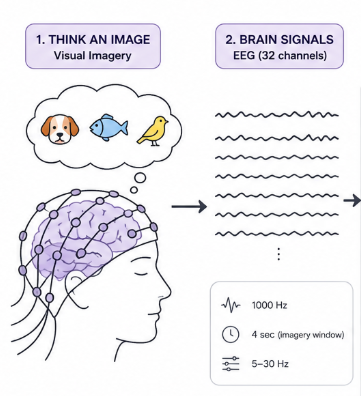
\includegraphics[width=0.86\linewidth]{figures/image2.png}
  \caption{Concept of visual-imagery decoding. The user mentally pictures an
  object (e.g., dog, fish, bird); 32-channel EEG is recorded at 1000\,Hz and
  band-pass filtered to 5--30\,Hz; the decoder classifies the 4\,s imagery
  window.}
  \label{fig:concept}
\end{figure}

% =====================================================================
%  III. RELATED WORK
% =====================================================================
\section{Related Work}
We organize prior work into four strands: decoding backbones, visual-imagery
and semantic decoding, cross-subject and transfer learning, and clinical
BCIs for ALS and locked-in syndrome.

\subsection{Decoding Backbones}
EEGNet~\cite{lawhern2018} is a compact CNN using depthwise and separable
convolutions that generalizes across many EEG paradigms (P300, error
potentials, motor imagery, SSVEP); it is the deep model used in our dataset's
own validation and therefore our natural baseline. Classical pipelines are
well surveyed by Lotte \textit{et al.}~\cite{lotte2007}, whose review of
feature extraction and classification (CSP, LDA, SVM, $k$-NN) frames the
CSP+KNN baseline that the dataset also reports. The EEG
Conformer~\cite{song2022} combines a convolutional front-end with
self-attention and reached state-of-the-art results on motor-imagery and
emotion tasks, making it a strong candidate backbone. EEG-Deformer%
~\cite{ding2024} adds a hierarchical coarse-to-fine temporal module and an
information-purification block, matching or beating the state of the art on
attention, fatigue, and workload tasks while producing neurophysiologically
meaningful attention maps. Most relevant to our lightweight goal,
DBConformer~\cite{wang_db2025} models temporal and inter-channel dependencies
in separate branches with a channel-attention module and outperforms ten or
more baselines using roughly eight times fewer parameters than the original
Conformer. DreamEEG builds on this CNN + Transformer lineage but adds an
explicit variance-coupled dual-stream design.

\subsection{Visual-Imagery and Semantic Decoding}
The dataset of Gao \textit{et al.}~\cite{gao2026} is, to our knowledge, the
first open, VI-focused benchmark of its scale, and its EEGNet baseline
(75\% / 62\% on objects, within-subject) sets the bar for this work. The
breadth of the imagery-decoding field is illustrated by
EEG2Video~\cite{eeg2video2024}, which reconstructs dynamic visual perception
from EEG. For imagery specifically, Wilson \textit{et al.}~\cite{wilson2023}
released an open 128-channel semantic-concept dataset used as a comparison
point by our target dataset, and Pan \textit{et al.}~\cite{pan2024} pushed VI
toward spelling by classifying 29 characters from visual imagery. Kilmarx
\textit{et al.}~\cite{kilmarx2024} systematically evaluated VI as a control
strategy and reported that it is feasible but limited by high variability and
modest accuracy, precisely the motivation for stronger decoders. Lee
\textit{et al.}~\cite{lee2020} established VI and imagined speech as
intuitive, endogenous paradigms, and Sousa \textit{et al.}~\cite{sousa2017}
showed that pure VI alone can provide three classes of control for non-motor
disorders. On the neuroscience side, Rybar \textit{et al.}~\cite{rybar2025}
showed imagined semantic categories are decodable from simultaneous EEG and
fNIRS, and Huang \textit{et al.}~\cite{huang2024} used a spatio-temporal
capsule network, arguing that semantic decoding generalizes better than
low-level visual-feature decoding.

\subsection{Cross-Subject and Transfer Learning}
Because the practical bottleneck for VI-BCIs is per-user calibration,
transfer learning is central to our staged plan. Wang
\textit{et al.}~\cite{wang_group2025} built a lightweight semantic-decoding
network that explicitly balances group-level commonality against individual
variability via group-to-individual transfer, the closest published idea to
our own generalization goal. Junqueira \textit{et al.}~\cite{junqueira2024}
showed that Euclidean Alignment is a simple, low-cost normalization that
reliably improves cross-subject decoding with deep networks, which is why we
adopt it as a first alignment step. Wu \textit{et al.}~\cite{wu2022} provide
a tutorial that organizes EEG transfer learning into cross-subject and
cross-session settings and into instance-, feature-, and parameter-based
methods, giving us a menu of adaptation strategies.

\subsection{Clinical BCIs for ALS and Locked-In Syndrome}
Birbaumer \textit{et al.}~\cite{birbaumer1999} gave the first proof that
paralysed users, including people with ALS, could spell by self-regulating
slow cortical potentials with only a scalp EEG cap. K\"ubler
\textit{et al.}~\cite{kubler2005} showed people severely disabled by ALS
could control a sensorimotor-rhythm BCI, and Nijboer
\textit{et al.}~\cite{nijboer2008} took a P300 speller into ALS patients'
homes with accuracy sustained over months. Moving to invasive systems,
Vansteensel \textit{et al.}~\cite{vansteensel2016} let a locked-in ALS
patient type at home through a fully implanted BCI, and Willett
\textit{et al.}~\cite{willett2023} decoded attempted speech at about 62 words
per minute. These systems are powerful but invasive and heavily per-user
calibrated; our work targets a non-invasive, lightweight alternative built on
visual rather than motor or speech imagery.

% =====================================================================
%  IV. DATASET
% =====================================================================
\section{Dataset}
All experiments use the openly released visual-imagery EEG dataset of
Gao \textit{et al.}~\cite{gao2026}, published in \textit{Scientific Data}.
Its key properties are summarized in Table~\ref{tab:dataset}.

\begin{table}[t]
  \caption{Summary of the Visual-Imagery EEG Dataset~\cite{gao2026}}
  \label{tab:dataset}
  \centering
  \renewcommand{\arraystretch}{1.25}
  \begin{tabular}{@{}p{0.24\linewidth} p{0.66\linewidth}@{}}
    \toprule
    \textbf{Property} & \textbf{Value} \\
    \midrule
    Source        & Gao \textit{et al.} (2026), \textit{Scientific Data};
                    open; VI-focused; new (no prior decoding work) \\
    Participants  & 22 healthy; aged 20--23; 5 female; two sessions on
                    different days (19 of 22 completed both) \\
    Recording     & 32-channel wireless system; 1000\,Hz; 10--20 layout
                    (AFz ground, CPz reference); shielded room \\
    Stimuli       & 10 images; 3 categories (figures, animals, objects) \\
    Trial (17\,s) & fixation 3\,s $\rightarrow$ image 4\,s $\rightarrow$
                    mask 2\,s $\rightarrow$ imagery 4\,s $\rightarrow$ rest;
                    the 4\,s imagery window is decoded \\
    Task          & 3-class within a category (e.g., dog vs.\ fish vs.\
                    bird); chance $=33\%$; 120/120/160 trials \\
    Preproc.      & 5--30\,Hz band-pass; common average reference;
                    ICA (Picard) + ICLabel; 4\,s epochs \\
    Quality       & open BIDS format; raw + preprocessed; baseline code
                    (MNE, PyTorch) \\
    \bottomrule
  \end{tabular}
\end{table}

The decoding target is deliberately narrow and well defined: a three-way,
within-category classification of the 4\,s imagery epoch, giving a 33\%
chance level. Recordings span two sessions on different days, which lets us
measure day-to-day stability, and the open BIDS packaging with reference
code makes faithful baseline reproduction possible. The dataset and its
descriptor paper are publicly available.\footnote{Dataset:
\url{https://figshare.com/articles/dataset/EEG_Dataset_for_Visual_Imagery/30227503};
descriptor: \url{https://www.nature.com/articles/s41597-025-06512-5}.}

Fig.~\ref{fig:eeg} shows the general non-invasive EEG acquisition setup that
underlies this recording paradigm.

\begin{figure}[t]
  \centering
  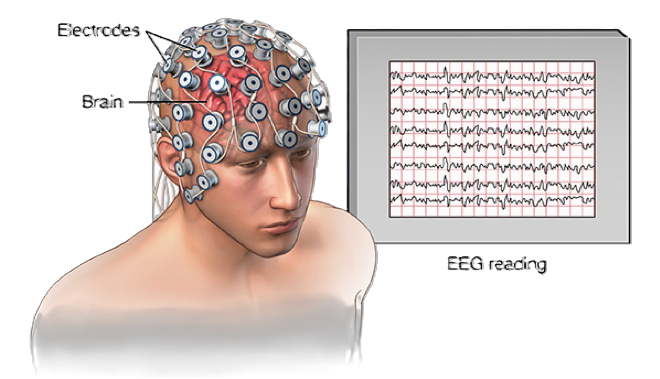
\includegraphics[width=0.9\linewidth]{figures/image1.png}
  \caption{Non-invasive scalp EEG acquisition: an electrode cap records
  cortical activity that is digitized into multi-channel time series (the
  ``EEG reading''). The study dataset uses a 32-channel, 10--20 montage.}
  \label{fig:eeg}
\end{figure}

% =====================================================================
%  V. RESEARCH OBJECTIVES
% =====================================================================
\section{Research Objectives}
The project pursues six objectives, ordered from the core technical goal to
its clinical justification.

\begin{enumerate}
  \item \textbf{Stronger decoder (primary).} Design a combined
        CNN--Transformer that beats the EEGNet baseline.
  \item \textbf{Fix the weakest task.} Lift object-category accuracy
        ($\sim$62\%) toward the level of figures and animals ($\sim$75\%).
  \item \textbf{Lightweight and practical.} Keep few parameters, train on a
        single GPU, and remain deployable for real assistive use.
  \item \textbf{Stable over time.} Stay consistent from day to day
        (session 1 $\rightarrow$ session 2).
  \item \textbf{Generalize to new users.} Reduce per-user calibration via
        transfer learning and alignment.
  \item \textbf{Clinical relevance.} Be reliable enough to aid ALS /
        locked-in communication.
\end{enumerate}

% =====================================================================
%  VI. PROPOSED METHOD
% =====================================================================
\section{Proposed Method}

\subsection{Hypothesis}
Our working hypothesis is twofold. First, not all electrodes contribute
equally to VI decoding; we therefore begin by identifying which
probes/channels are most informative for this specific problem. Second, on
top of that channel evidence, a \emph{customized} hybrid model that jointly
models first- and second-order signal statistics will extract more
discriminative structure than a single-stream CNN, and will do so most where
the baseline is weakest (the object category).

\subsection{Architecture}
DreamEEG (Fig.~\ref{fig:arch}) takes a preprocessed EEG epoch of
$32\ \text{channels} \times 4\ \text{s}$, band-pass filtered to 5--30\,Hz,
and passes it through three stages.

\paragraph{Shared front-end} A \emph{multi-scale temporal convolution} with
parallel kernels of length 32, 64, 96, and 128 captures rhythmic structure
at several time scales simultaneously. A \emph{depthwise spatial convolution}
($C\times1$), followed by batch normalization and an ELU nonlinearity, then
learns channel/spatial filters analogous to spatial patterns.

\paragraph{Variance-coupled dual-stream encoder (key edge)} The shared
features branch into two complementary streams:
\begin{itemize}
  \item a \textbf{first-order stream} using a mean pool ($P_{\mu}$) that
        summarizes average activation, and
  \item a \textbf{second-order stream} using a log-variance pool
        ($P_{\sigma^2}$) that captures band-power / signal energy, a feature
        long known to be informative for imagery EEG.
\end{itemize}
Each stream is refined by a stack of four \emph{gated dual-attention
Transformer} blocks that apply both spatial and temporal attention gates,
letting the model weight informative channels and time points.

\paragraph{Fusion head} The two stream representations are concatenated,
passed through a convolutional layer, and mapped by a softmax to the three
within-category classes (e.g., dog, fish, bird).

\begin{figure}[t]
  \centering
  \resizebox{0.99\linewidth}{!}{%
  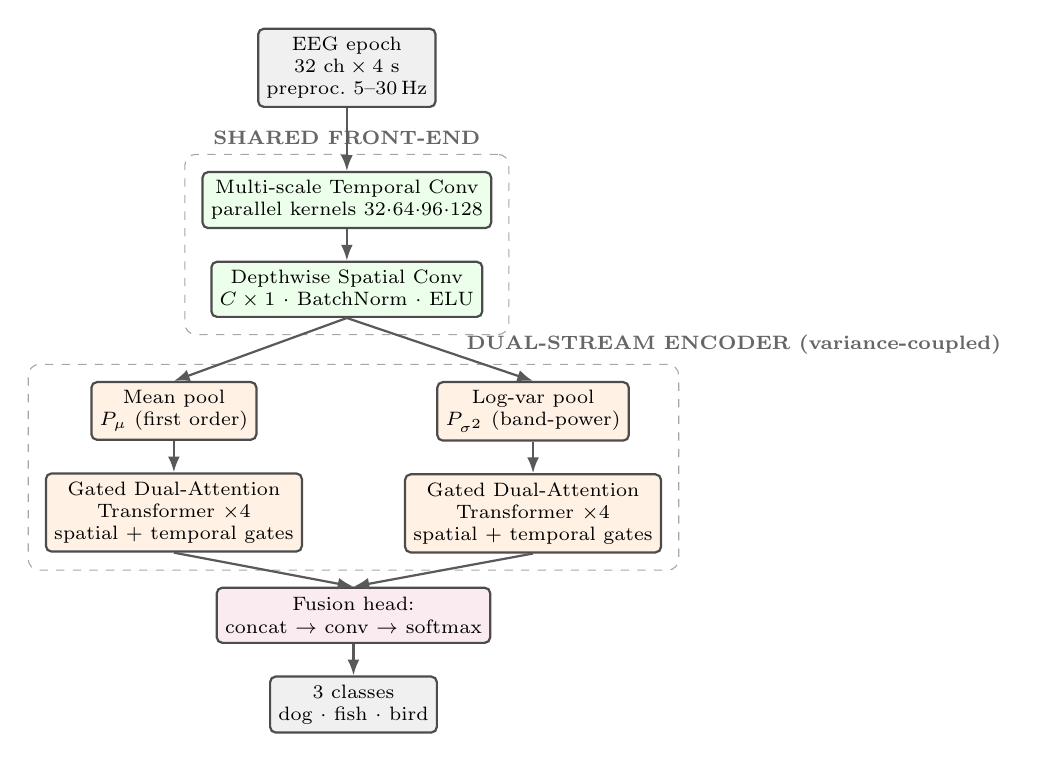
\begin{tikzpicture}[node distance=4mm and 6mm]
    % ---- Input ----
    \node[io] (in) {EEG epoch\\ $32\text{ ch}\times4\text{ s}$\\
                     preproc.\ 5--30\,Hz};

    % ---- Shared front-end ----
    \node[frontend, below=8mm of in] (ms) {Multi-scale Temporal Conv\\
                     parallel kernels 32$\cdot$64$\cdot$96$\cdot$128};
    \node[frontend, below=of ms] (dw) {Depthwise Spatial Conv\\
                     $C\times1$ $\cdot$ BatchNorm $\cdot$ ELU};

    % ---- Dual stream ----
    \node[stream, below left=8mm and -6mm of dw]  (mp) {Mean pool\\
                     $P_{\mu}$ (first order)};
    \node[stream, below right=8mm and -6mm of dw] (vp) {Log-var pool\\
                     $P_{\sigma^2}$ (band-power)};
    \node[stream, below=of mp] (t1) {Gated Dual-Attention\\
                     Transformer $\times4$\\ spatial + temporal gates};
    \node[stream, below=of vp] (t2) {Gated Dual-Attention\\
                     Transformer $\times4$\\ spatial + temporal gates};

    % ---- Fusion head (centered below both Transformer streams) ----
    \node[head] (fus) at ($(t1)!0.5!(t2) + (0,-1.3cm)$)
                     {Fusion head:\\ concat $\rightarrow$ conv
                      $\rightarrow$ softmax};
    \node[io, below=of fus] (out) {3 classes\\ dog $\cdot$ fish $\cdot$ bird};

    % ---- Arrows ----
    \draw[ar] (in) -- (ms);
    \draw[ar] (ms) -- (dw);
    \draw[ar] (dw.south) -- (mp.north);
    \draw[ar] (dw.south) -- (vp.north);
    \draw[ar] (mp) -- (t1);
    \draw[ar] (vp) -- (t2);
    \draw[ar] (t1.south) -- (fus.north);
    \draw[ar] (t2.south) -- (fus.north);
    \draw[ar] (fus) -- (out);

    % ---- Group boxes ----
    \begin{scope}[on background layer]
      \node[grp, fit=(ms)(dw), label={[lbl]above:SHARED FRONT-END}] {};
      \node[grp, fit=(mp)(vp)(t1)(t2),
            label={[lbl]above right:DUAL-STREAM ENCODER (variance-coupled)}] {};
    \end{scope}
  \end{tikzpicture}}
  \caption{The proposed DreamEEG architecture: a shared multi-scale
  convolutional front-end, a variance-coupled dual-stream encoder pairing a
  first-order (mean) and a second-order (log-variance / band-power) path,
  each refined by gated dual-attention Transformer blocks, and a fusion head
  producing the 3-class decision.}
  \label{fig:arch}
\end{figure}

The design keeps the parameter count modest, in the spirit of compact
decoders such as EEGNet and DBConformer, so that it remains single-GPU
trainable and deployable, in line with Objective~3.

% =====================================================================
%  VII. EVALUATION PLAN
% =====================================================================
\section{Evaluation Protocol and Staged Plan}

\subsection{The Bar to Beat}
The primary benchmark is the EEGNet baseline reported with the
dataset~\cite{gao2026}, evaluated within-subject on the 3-class
within-category task (chance $=33\%$). Table~\ref{tab:baseline} lists the
per-category accuracies. Objects, at 62.0\%, are the clear weak spot and are
therefore our main improvement target: the hardest but most useful case.

\begin{table}[t]
  \caption{EEGNet Baseline to Beat (Within-Subject)~\cite{gao2026}}
  \label{tab:baseline}
  \centering
  \renewcommand{\arraystretch}{1.25}
  \begin{tabular}{@{}lcc@{}}
    \toprule
    \textbf{Category} & \textbf{Accuracy} & \textbf{Chance} \\
    \midrule
    Figures & 75.1\% & 33\% \\
    Animals & 75.8\% & 33\% \\
    \textbf{Objects} & \textbf{62.0\%} & 33\% \\
    \bottomrule
  \end{tabular}
\end{table}

Evaluation uses the same 22 subjects, 32 channels at 1000\,Hz, and two
sessions provided in the open BIDS release with baseline code, so that our
numbers are directly comparable.

\subsection{Staged Plan}
The plan is deliberately staged so that each step yields a usable result even
if a later step underperforms, which keeps risk low against the project
timeline.
\begin{enumerate}
  \item \textbf{Reproduce the baseline.} Re-run the authors' within-subject
        EEGNet and CSP+KNN to confirm our pipeline matches their reported
        numbers, validating that we read and preprocess the data correctly.
  \item \textbf{Build and tune DreamEEG.} Develop the hybrid CNN--Transformer,
        our core contribution, and tune it to beat the within-subject
        baseline, with particular attention (and augmentation) on the weak
        object category.
  \item \textbf{Cross-subject benchmark.} Move to leave-one-subject-out
        (LOSO) evaluation (train on 21 subjects, test on the held-out one)
        and add Euclidean Alignment~\cite{junqueira2024} as a first,
        low-cost step to close the expected generalization gap. No
        cross-subject benchmark exists on this dataset yet, so quantifying it
        is itself a contribution.
  \item \textbf{Transfer learning and cross-session test.} Apply light
        domain adaptation / fine-tuning~\cite{wu2022} to measure how few
        target trials are needed for acceptable accuracy, and train on
        session 1 / test on session 2 (19 two-session subjects) to report
        temporal stability.
\end{enumerate}

Throughout, we report accuracy, macro-F1, and Cohen's $\kappa$, together with
per-category results and confusion-matrix structure, in the within-subject,
cross-session, and cross-subject (LOSO) settings, alongside the parameter
count to document the lightweight goal.

% =====================================================================
%  VIII. EXPECTED OUTCOMES & CONCLUSION
% =====================================================================
\section{Expected Outcomes and Conclusion}
We expect DreamEEG to deliver a stronger yet lighter visual-imagery decoder
that surpasses the EEGNet baseline, with the largest gains on the currently
weak object category, while remaining stable across sessions and more
transferable across users. If achieved, such a decoder moves VI-based BCIs a
concrete step closer to being a dependable communication channel. For a
person with ALS or locked-in syndrome, a brain--computer interface could then
actually help restore a voice.

This midterm report has established the clinical motivation, isolated the
decoder as the true bottleneck, described the open VI dataset and its
baseline, and specified the DreamEEG architecture together with a staged plan
to validate it. The next phase focuses on baseline reproduction and the first
full training runs of the proposed model.

% =====================================================================
%  REFERENCES  (embedded -- no external .bib required)
% =====================================================================
\begin{thebibliography}{99}

\bibitem{birbaumer1999}
N.~Birbaumer, N.~Ghanayim, T.~Hinterberger, I.~Iversen, B.~Kotchoubey,
A.~K\"ubler, J.~Perelmouter, E.~Taub, and H.~Flor, ``A spelling device for
the paralysed,'' \textit{Nature}, vol.~398, no.~6725, pp.~297--298, 1999,
doi: 10.1038/18581.

\bibitem{vansteensel2016}
M.~J. Vansteensel \textit{et al.}, ``Fully implanted brain--computer
interface in a locked-in patient with ALS,'' \textit{New England Journal of
Medicine}, vol.~375, no.~21, pp.~2060--2066, 2016,
doi: 10.1056/NEJMoa1608085.

\bibitem{gao2026}
J.~Gao \textit{et al.}, ``An EEG dataset for visual imagery-based
brain--computer interface,'' \textit{Scientific Data}, vol.~13, art.~194,
2026, doi: 10.1038/s41597-025-06512-5.

\bibitem{lawhern2018}
V.~J. Lawhern, A.~J. Solon, N.~R. Waytowich, S.~M. Gordon, C.~P. Hung, and
B.~J. Lance, ``EEGNet: A compact convolutional neural network for EEG-based
brain--computer interfaces,'' \textit{Journal of Neural Engineering},
vol.~15, no.~5, art.~056013, 2018, doi: 10.1088/1741-2552/aace8c.

\bibitem{lotte2007}
F.~Lotte, M.~Congedo, A.~L\'ecuyer, F.~Lamarche, and B.~Arnaldi, ``A review
of classification algorithms for EEG-based brain--computer interfaces,''
\textit{Journal of Neural Engineering}, vol.~4, no.~2, pp.~R1--R13, 2007,
doi: 10.1088/1741-2560/4/2/R01.

\bibitem{song2022}
Y.~Song, Q.~Zheng, B.~Liu, and X.~Gao, ``EEG Conformer: Convolutional
Transformer for EEG decoding and visualization,'' \textit{IEEE Transactions
on Neural Systems and Rehabilitation Engineering}, vol.~31, pp.~710--719,
2023, doi: 10.1109/TNSRE.2022.3230250.

\bibitem{ding2024}
Y.~Ding \textit{et al.}, ``EEG-Deformer: A dense convolutional Transformer
for brain--computer interfaces,'' \textit{arXiv preprint}
arXiv:2405.00719, 2024.

\bibitem{wang_db2025}
Z.~Wang \textit{et al.}, ``DBConformer: Dual-branch convolutional Transformer
for EEG decoding,'' \textit{arXiv preprint} arXiv:2506.21140, 2025.

\bibitem{eeg2video2024}
X.~Liu \textit{et al.}, ``EEG2Video: Towards decoding dynamic visual
perception from EEG signals,'' in \textit{Advances in Neural Information
Processing Systems (NeurIPS)}, 2024.

\bibitem{wilson2023}
H.~Wilson, M.~Golbabaee, M.~J. Proulx, S.~Charles, and E.~O'Neill,
``EEG-based BCI dataset of semantic concepts for imagination and perception
tasks,'' \textit{Scientific Data}, vol.~10, 2023,
doi: 10.1038/s41597-023-02287-9.

\bibitem{pan2024}
H.~Pan, W.~Song, L.~Li, and X.~Qin, ``The design and implementation of a
multi-character classification scheme based on EEG signals of visual
imagery,'' \textit{Cognitive Neurodynamics}, vol.~18, pp.~2299--2309, 2024,
doi: 10.1007/s11571-024-10087-z.

\bibitem{kilmarx2024}
J.~Kilmarx, I.~Tashev, J.~del~R. Mill\'an, J.~Sulzer, and J.~Lewis-Peacock,
``Evaluating the feasibility of visual imagery for an EEG-based
brain--computer interface,'' \textit{IEEE Transactions on Neural Systems and
Rehabilitation Engineering}, vol.~32, pp.~2209--2219, 2024,
doi: 10.1109/TNSRE.2024.3410870.

\bibitem{lee2020}
S.~H. Lee, M.~Lee, and S.~W. Lee, ``Neural decoding of imagined speech and
visual imagery as intuitive paradigms for BCI communication,'' \textit{IEEE
Transactions on Neural Systems and Rehabilitation Engineering}, vol.~28,
no.~12, pp.~2647--2659, 2020, doi: 10.1109/TNSRE.2020.3040289.

\bibitem{sousa2017}
T.~Sousa \textit{et al.}, ``Pure visual imagery as a potential approach to
achieve three classes of control for implementation of BCI in non-motor
disorders,'' \textit{Journal of Neural Engineering}, vol.~14, no.~4,
art.~046026, 2017, doi: 10.1088/1741-2552/aa70ac.

\bibitem{rybar2025}
M.~Rybar, R.~Poli, and I.~Daly, ``Simultaneous EEG and fNIRS recordings for
semantic decoding of imagined animals and tools,'' \textit{Scientific Data},
vol.~12, 2025, doi: 10.1038/s41597-025-04967-0.

\bibitem{huang2024}
J.~Huang, Y.~Chang, W.~Li, J.~Tong, and S.~Du, ``A spatio-temporal capsule
neural network with self-correlation routing for EEG decoding of semantic
concepts,'' \textit{Sensors}, vol.~24, no.~18, art.~5988, 2024,
doi: 10.3390/s24185988.

\bibitem{wang_group2025}
X.~Wang \textit{et al.}, ``A lightweight semantic decoding network with
group-to-individual transfer learning for EEG-based visual recognition,''
\textit{Neurocomputing}, 2025.

\bibitem{junqueira2024}
B.~Junqueira, B.~Aristimunha, S.~Chevallier, and R.~de~Camargo, ``A
systematic evaluation of Euclidean alignment with deep learning for EEG
decoding,'' \textit{Journal of Neural Engineering}, 2024,
doi: 10.1088/1741-2552/ad4f18.

\bibitem{wu2022}
D.~Wu, X.~Jiang, and R.~Peng, ``Transfer learning for motor imagery based
brain--computer interfaces: A tutorial,'' \textit{Neural Networks},
vol.~153, pp.~235--253, 2022, doi: 10.1016/j.neunet.2022.06.008.

\bibitem{kubler2005}
A.~K\"ubler \textit{et al.}, ``Patients with ALS can use sensorimotor rhythms
to operate a brain--computer interface,'' \textit{Neurology}, vol.~64,
no.~10, pp.~1775--1777, 2005, doi: 10.1212/01.WNL.0000158616.43002.6D.

\bibitem{nijboer2008}
F.~Nijboer \textit{et al.}, ``A P300-based brain--computer interface for
people with amyotrophic lateral sclerosis,'' \textit{Clinical
Neurophysiology}, vol.~119, no.~8, pp.~1909--1916, 2008,
doi: 10.1016/j.clinph.2008.03.034.

\bibitem{willett2023}
F.~R. Willett \textit{et al.}, ``A high-performance speech neuroprosthesis,''
\textit{Nature}, vol.~620, pp.~1031--1036, 2023,
doi: 10.1038/s41586-023-06377-x.

\end{thebibliography}

\end{document}
